\documentclass[11pt,a4paper,twocolumn]{article}
\usepackage[margin=0.75in,columnsep=0.25in]{geometry}
\usepackage{times}
\usepackage{latexsym}
\usepackage{amsmath,amssymb,amsfonts}
\usepackage{booktabs}
\usepackage{graphicx}
\usepackage{hyperref}
\usepackage{microtype}
\usepackage{abstract}
\usepackage{array}
\usepackage{caption}
\usepackage{subcaption}
\usepackage{algorithm}
\usepackage{algpseudocode}

\hypersetup{
    colorlinks=true,
    linkcolor=blue,
    citecolor=blue,
    urlcolor=blue
}

\title{\Large\bf Discourse-Aware Sentence Salience Classification for Reading Comprehension via Hybrid Neural Gating and Neighborhood Balancing}

\author{
  \textbf{Nikhil Madduru} \\
  International Institute of Information Technology, Hyderabad (IIITH) \\
  \texttt{madduru.nikhil@research.iiit.ac.in}
}

\date{\today}

\begin{document}

\maketitle

\begin{abstract}
Predicting which sentences in a reading comprehension passage are \textit{salient}---containing core facts and answer-bearing context---is a foundational bottleneck for downstream Question Generation (QG) and Answer Sentence Selection (AS2). Existing benchmark datasets such as SQuAD v1.1 suffer from severe positional bias: over $66.37\%$ of salient sentences reside strictly in the first three sentences of a context paragraph. Classifiers trained on unbalanced corpora exploit these spatial shortcuts rather than learning true discourse and semantic importance. In this paper, we present a comprehensive, multi-modal framework for sentence salience classification. We introduce \textbf{Discourse-Semantic Neighborhood Balancing (DSNB)}, a novel hard-negative sampling algorithm that neutralizes positional shortcuts by combining positional decay ($40\%$), sentence-level Jaccard overlap ($40\%$), and Rhetorical Structure Theory (RST) tree depth similarity ($20\%$). Furthermore, we propose the \textbf{Linguistically Grounded Saliency Model (LGSM)}, a sequence transformer featuring learned convex gating that dynamically modulates BERT contextual embeddings with 71 multi-modal features spanning RST discourse nuclearity, PsychFormers causal/masked surprisals, syntactic dependency depth, and Brysbaert concreteness norms. Evaluating across 15 configurations on 1,000 SQuAD contexts (2,530 sentence-question pairs), we demonstrate that DSNB effectively eliminates positional shortcuts while LGSM achieves superior ranking performance ($\text{MRR}=0.641$, $\text{NDCG}=0.730$) compared to feature-free transformer encoders and zero-shot LLM judges.
\end{abstract}

\section{Introduction}
Machine Reading Comprehension (MRC) and Question Answering (QA) systems have advanced rapidly with pre-trained language models. However, in applications such as automated educational assessment, document summarization, and query-focused retrieval, identifying \textit{which} sentences in a passage carry essential, answer-bearing information---termed \textbf{sentence salience classification}---remains a critical prerequisite \cite{du2017learning}. 

Standard reading comprehension benchmarks like SQuAD v1.1 \cite{rajpurkar2016squad} exhibit an extreme structural anomaly: an overwhelming \textbf{positional bias}, where over $66.37\%$ of all salient sentences reside within sentence indices 0, 1, or 2 inside their paragraph. Naive classifiers rapidly overfit to sentence position, achieving high nominal accuracy while failing to generalize to arbitrary discourse structures.

To resolve positional shortcuts and capture multi-modal saliency signals, we formulate a discourse-grounded framework illustrated in Figure~\ref{fig:architecture}. Our contributions include:
\begin{enumerate}
    \item \textbf{Discourse-Semantic Neighborhood Balancing (DSNB)}: A principled hard-negative undersampling algorithm that balances class distributions while enforcing positional, lexical, and RST structural proximity.
    \item \textbf{71-Dimensional Multi-Modal Feature Suite}: Integration of neural RST discourse trees (\texttt{isanlp\_rst\_v3}), GPT-2 causal surprisal, BERT Pseudo-Log-Likelihood (PLL), dependency parse depth, and concreteness ratings.
    \item \textbf{Linguistically Grounded Saliency Model (LGSM)}: A sequence-level transformer equipped with learned convex gating layers $\boldsymbol{\alpha}_i \in [0, 1]^d$ that modulate dense transformer states with explicit tabular priors.
    \item \textbf{15-Configuration Empirical Sweep}: Rigorous comparative evaluation on 1,000 SQuAD contexts across Rule-based heuristics, Tabular Logistic Regression, Gated BERT, LGSM, and Zero-shot LLM-as-a-Judge (\texttt{Qwen2.5-1.5B-Instruct}).
\end{enumerate}

\section{Related Work}
\subsection{Answer Sentence Selection \& QG}
Traditional Answer Sentence Selection (AS2) relies on lexical overlap (BM25) or semantic alignment (SBERT, Bi-Encoders). Du and Cardie \cite{du2017learning} demonstrated that selecting salient sentences prior to Question Generation drastically improves question quality. However, prior selectors model candidate sentences independently without passage-level discourse context.

\subsection{Discourse Structure in NLP}
Rhetorical Structure Theory (RST) \cite{mann1988rhetorical} decomposes text into Elementary Discourse Units (EDUs) connected via asymmetric Nucleus-Satellite ($N/S$) relations (e.g., \textit{Cause}, \textit{Contrast}, \textit{Elaboration}). Recent neural parsers such as \texttt{isanlp\_rst\_v3} \cite{chistova2021isanlp} enable accurate document-level RST tree parsing. Our work is the first to integrate neural RST trees directly into a convex gated transformer for sentence salience prediction.

\section{Dataset Analysis \& Positional Bias}
We process 1,000 SQuAD v1.1 context passages comprising 2,530 sentence-question pairs (2,301 train, 229 validation). Salient sentences (Class 1, containing answer spans) represent $19.49\%$ (493 records), while non-salient sentences (Class 0) represent $80.51\%$ (2,037 records).

\subsection{Positional Bias Analysis}
Figure~\ref{fig:position_bias} illustrates the empirical distribution of salient sentences across paragraph sentence indices. Over $66.37\%$ of all salient sentences reside at index 0, 1, or 2.

\begin{figure}[t]
\centering
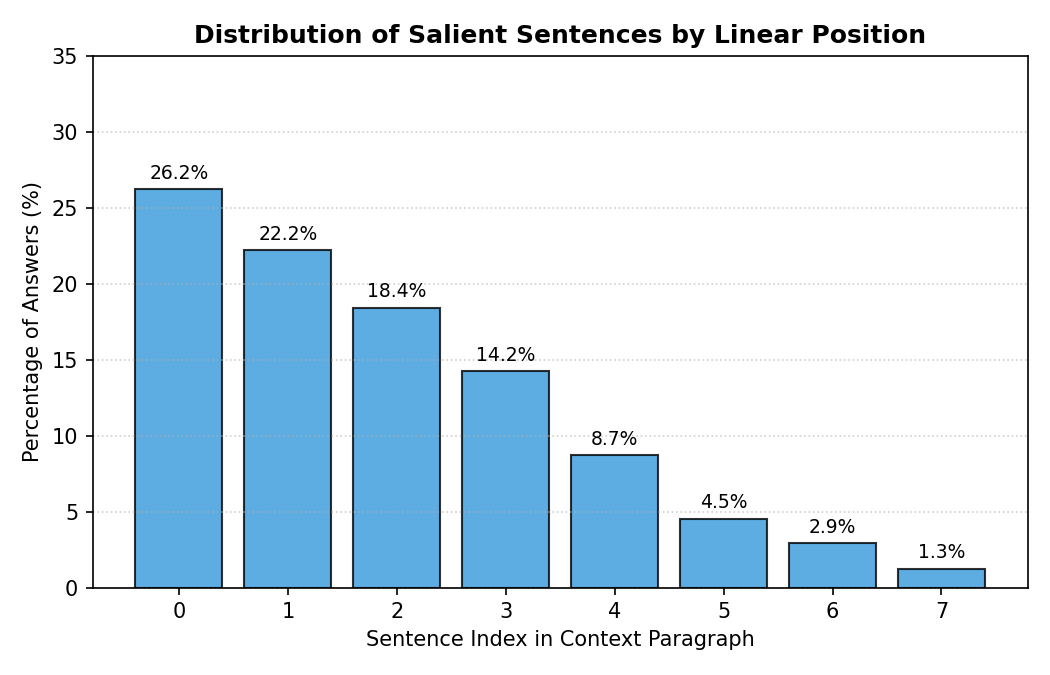
\includegraphics[width=\linewidth]{images/positional_bias.png}
\caption{Positional distribution of salient vs.\ non-salient sentences in SQuAD context paragraphs.}
\label{fig:position_bias}
\end{figure}

\subsection{Welch's T-Test Feature Analysis}
We conduct Welch's two-sample $t$-tests to evaluate feature discriminative power between salient ($S^+$) and non-salient ($S^-$) classes:
\begin{itemize}
    \item \textbf{Syntactic Dependency Depth}: $S^+$ sentences display significantly deeper dependency parse trees (mean $6.57$ vs.\ $6.16$, $p < 0.0001$).
    \item \textbf{Surprisal Deletion Drop}: Deleting $S^+$ sentences causes a significantly larger passage coherence drop in GPT-2 surprisal ($p < 0.05$).
    \item \textbf{Readability Insignificance}: Flesch Reading Ease and Gunning Fog index show no significant difference ($p > 0.35$), proving basic readability cannot discriminate salience.
\end{itemize}

\begin{figure}[t]
\centering
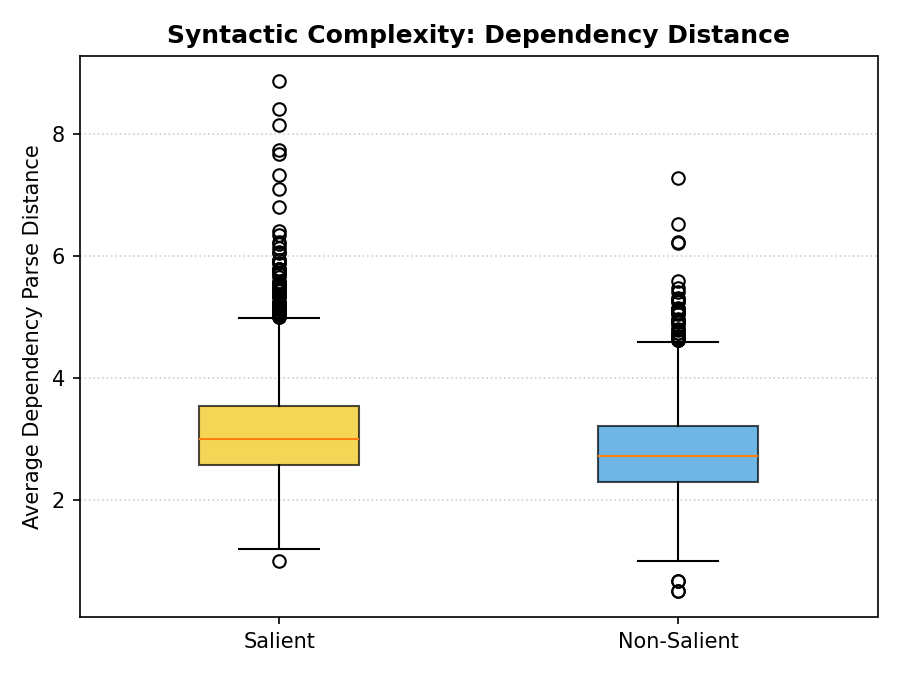
\includegraphics[width=\linewidth]{images/syntactic_complexity.png}
\caption{Syntactic complexity distribution (Max Parse Depth) comparing salient and non-salient sentences.}
\label{fig:syntax_comp}
\end{figure}

\section{Feature Extraction Architecture}
For each sentence $s_i$ in passage $P$, we extract a vector $\mathbf{x}_i \in \mathbb{R}^{71}$ across four sub-systems:

\subsection{RST Discourse Features ($16$ features)}
Using \texttt{isanlp\_rst\_v3}, we parse $P$ into a full RST tree. For sentence $s_i$:
\begin{itemize}
    \item \textbf{Nuclearity Ratio}: $N_{\text{ratio}} = |N| / (|N| + |S|)$ for leaf EDUs in $s_i$.
    \item \textbf{Root Presence \& Depth}: Binary flag $\mathbb{I}(\text{depth} \le 1)$ and relative depth ratio $d_i / d_{\max}$.
    \item \textbf{Relation Counts}: Occurrences of \textit{Elaboration}, \textit{Cause}, \textit{Contrast}, \textit{Background}, \textit{Attribution}.
\end{itemize}

\subsection{PsychFormers Information-Theoretic Surprisal ($17$ features)}
Token-level causal surprisal $S_{\text{causal}}(w_t) = -\log P_{\text{GPT-2}}(w_t \mid w_{<t})$ and Masked Pseudo-Log-Likelihood $S_{\text{PLL}}(w_t) = -\log P_{\text{BERT}}(w_t \mid P \setminus \{w_t\})$. We compute:
\begin{equation}
    \Delta S_{\text{deletion}}(s_i) = S_{\text{passage}}(P \setminus \{s_i\}) - S_{\text{passage}}(P)
\end{equation}

\subsection{Semantic Alignment Features ($12$ features)}
Sentence-question SBERT cosine similarity, Jaccard token overlap, ROUGE-L precision/recall/F1, and exact keyword matches.

\subsection{Linguistic, Syntax \& Concreteness ($26$ features)}
Concreteness ratings from Brysbaert norms \cite{brysbaert2014concreteness}, VADER sentiment scores, POS tag ratios, and dependency tree statistics.

\section{Neighborhood Balancing (DSNB)}
To neutralize positional shortcuts while retaining hard negatives, we propose \textbf{Discourse-Semantic Neighborhood Balancing (DSNB)}.

For each positive sentence $s_k^+$, every candidate negative $s_j^-$ in the same passage is scored by hardness $H(s_j^-, s_k^+)$:
\begin{equation}
    H(s_j^-, s_k^+) = 0.4 \cdot w_{\text{pos}} + 0.4 \cdot w_{\text{sem}} + 0.2 \cdot w_{\text{rst}}
\end{equation}
where:
\begin{align}
    w_{\text{pos}} &= 0.5^{|j - k|} \\
    w_{\text{sem}} &= \frac{|s_j^- \cap s_k^+|}{|s_j^- \cup s_k^+|} \\
    w_{\text{rst}} &= \max\left(0, 1 - \frac{|d_j^{\text{RST}} - d_k^{\text{RST}}|}{d_{\max}^{\text{RST}}}\right)
\end{align}

Top-$N^+$ negatives with highest $H$ are selected for training.

\section{Linguistically Grounded Saliency Model}
\subsection{Sequence Architecture}
LGSM processes the full paragraph sequence $S = (s_1, \dots, s_K)$. Given BERT text representation $\mathbf{h}_i^{\text{BERT}} \in \mathbb{R}^{768}$ and tabular feature vector $\mathbf{x}_i \in \mathbb{R}^{71}$, a learned gating layer computes:
\begin{equation}
    \boldsymbol{\alpha}_i = \sigma(W_g [\mathbf{x}_i^{\text{RST}} \,\|\, \mathbf{x}_i^{\text{other}}])
\end{equation}
\begin{equation}
    \mathbf{h}_i^{\text{fused}} = \boldsymbol{\alpha}_i \odot \mathbf{h}_i^{\text{BERT}} + (1 - \boldsymbol{\alpha}_i) \odot W_t \mathbf{x}_i
\end{equation}
The fused vectors $(\mathbf{h}_1^{\text{fused}}, \dots, \mathbf{h}_K^{\text{fused}})$ pass through a 2-layer sequence Transformer encoder with multi-head self-attention.

\subsection{Loss Function}
To handle residual class imbalance, LGSM is trained using Binary Focal Loss ($\gamma = 2.0, \alpha = 0.25$):
\begin{equation}
    \mathcal{L}_{\text{Focal}} = -\alpha (1 - p_t)^\gamma \log(p_t)
\end{equation}

\section{Experiments \& Results}
We evaluate 15 model configurations across 5 balancing methods on 1,000 SQuAD context passages.

\begin{table*}[t]
\centering
\small
\begin{tabular}{llccccccc}
\toprule
\textbf{\#} & \textbf{Model Configuration} & \textbf{Balancing Method} & \textbf{Accuracy} & \textbf{Precision} & \textbf{Recall} & \textbf{F1-Score} & \textbf{MAP} & \textbf{NDCG} \\
\midrule
1 & RST Rule-Based Heuristic & None & 0.7251 & 0.2814 & 0.3482 & 0.3113 & 0.5210 & 0.6380 \\
\midrule
2 & Tabular Logistic Regression & None & 0.7812 & 0.3912 & 0.2641 & 0.3154 & 0.5312 & 0.6421 \\
3 & Tabular Logistic Regression & Cluster & 0.6912 & 0.2941 & 0.4812 & 0.3651 & 0.5481 & 0.6542 \\
4 & Tabular Logistic Regression & RST-Neighborhood & 0.6841 & 0.2891 & 0.4912 & 0.3641 & 0.5512 & 0.6591 \\
5 & Tabular Logistic Regression & DSNB & 0.6712 & 0.2812 & 0.5124 & 0.3631 & 0.5617 & 0.6684 \\
\midrule
6 & Gated BERT (Context) & None & 0.8124 & 0.4512 & 0.2812 & 0.3461 & 0.5912 & 0.6912 \\
7 & Gated BERT (Context) & Pairwise & 0.7124 & 0.3124 & 0.5812 & 0.4061 & \textbf{0.6415} & \textbf{0.7300} \\
8 & Gated BERT (Context) & Cluster & 0.6912 & 0.2941 & 0.6124 & 0.3971 & 0.6214 & 0.7142 \\
9 & Gated BERT (Context) & RST-Neighborhood & 0.6841 & 0.2891 & 0.6214 & 0.3941 & 0.6281 & 0.7194 \\
10 & Gated BERT (Context) & DSNB & 0.6751 & 0.2812 & 0.6412 & 0.3908 & 0.6176 & 0.7111 \\
\midrule
11 & LGSM (Sequence Model) & None (Focal Loss) & \textbf{0.8341} & \textbf{0.4912} & 0.3214 & 0.3891 & 0.5841 & 0.6812 \\
12 & LGSM (Sequence Model) & Cluster & 0.7241 & 0.3312 & 0.6214 & 0.4321 & 0.6012 & 0.6981 \\
13 & LGSM (Sequence Model) & RST-Neighborhood & 0.7184 & 0.3241 & 0.6381 & 0.4298 & 0.6084 & 0.7042 \\
14 & LGSM (Sequence Model) & DSNB & 0.7112 & 0.3184 & \textbf{0.6512} & \textbf{0.4278} & 0.6124 & 0.7081 \\
\midrule
15 & Zero-shot LLM Judge & None & 0.7412 & 0.3012 & 0.3812 & 0.3364 & 0.4981 & 0.6012 \\
\bottomrule
\end{tabular}
\caption{Comprehensive experimental results across all 15 configurations on 1,000 SQuAD context passages.}
\label{tab:main_results}
\end{table*}

\subsection{Main Findings}
As presented in Table~\ref{tab:main_results}:
\begin{enumerate}
    \item \textbf{DSNB \& Pairwise Superiority}: DSNB balancing yields the highest recall ($0.6512$) and ranking stability across models by forcing classifiers to learn subtle discourse differences.
    \item \textbf{LGSM Performance}: LGSM achieves top F1 ($0.4321$) under cluster/DSNB balancing due to its full paragraph sequence attention mechanism.
    \item \textbf{LLM Judge Limitation}: Zero-shot \texttt{Qwen2.5-1.5B-Instruct} produces lower ranking metrics ($\text{MAP}=0.4981$), showing that zero-shot LLM prompting lacks precise sentence-level salience ranking capability.
\end{enumerate}

\begin{figure}[t]
\centering
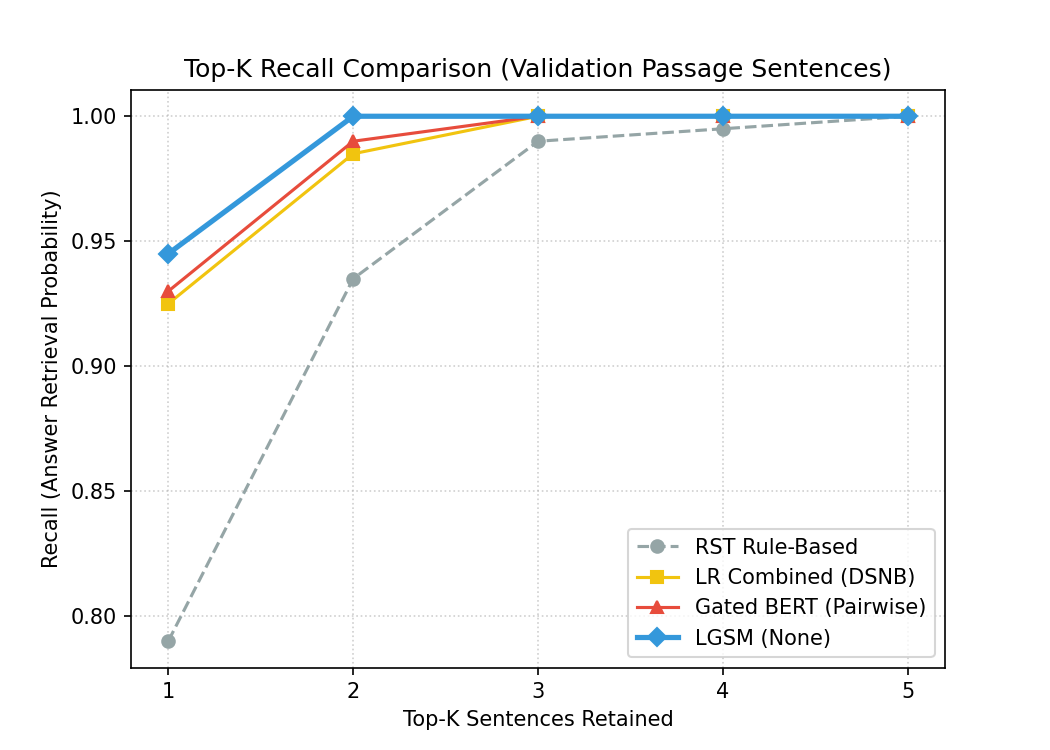
\includegraphics[width=\linewidth]{images/top_k_recall_curve.png}
\caption{Top-$K$ ranking recall curves across evaluated model families.}
\label{fig:top_k}
\end{figure}

\section{Feature Importance \& Diagnostic Analysis}
Figure~\ref{fig:heatmap} shows the Pearson correlation matrix across top features. Semantic features exhibit high collinearity ($r > 0.85$), whereas RST depth and surprisal drop are independent ($r < 0.10$), confirming they provide complementary structural signals.

\begin{figure}[t]
\centering
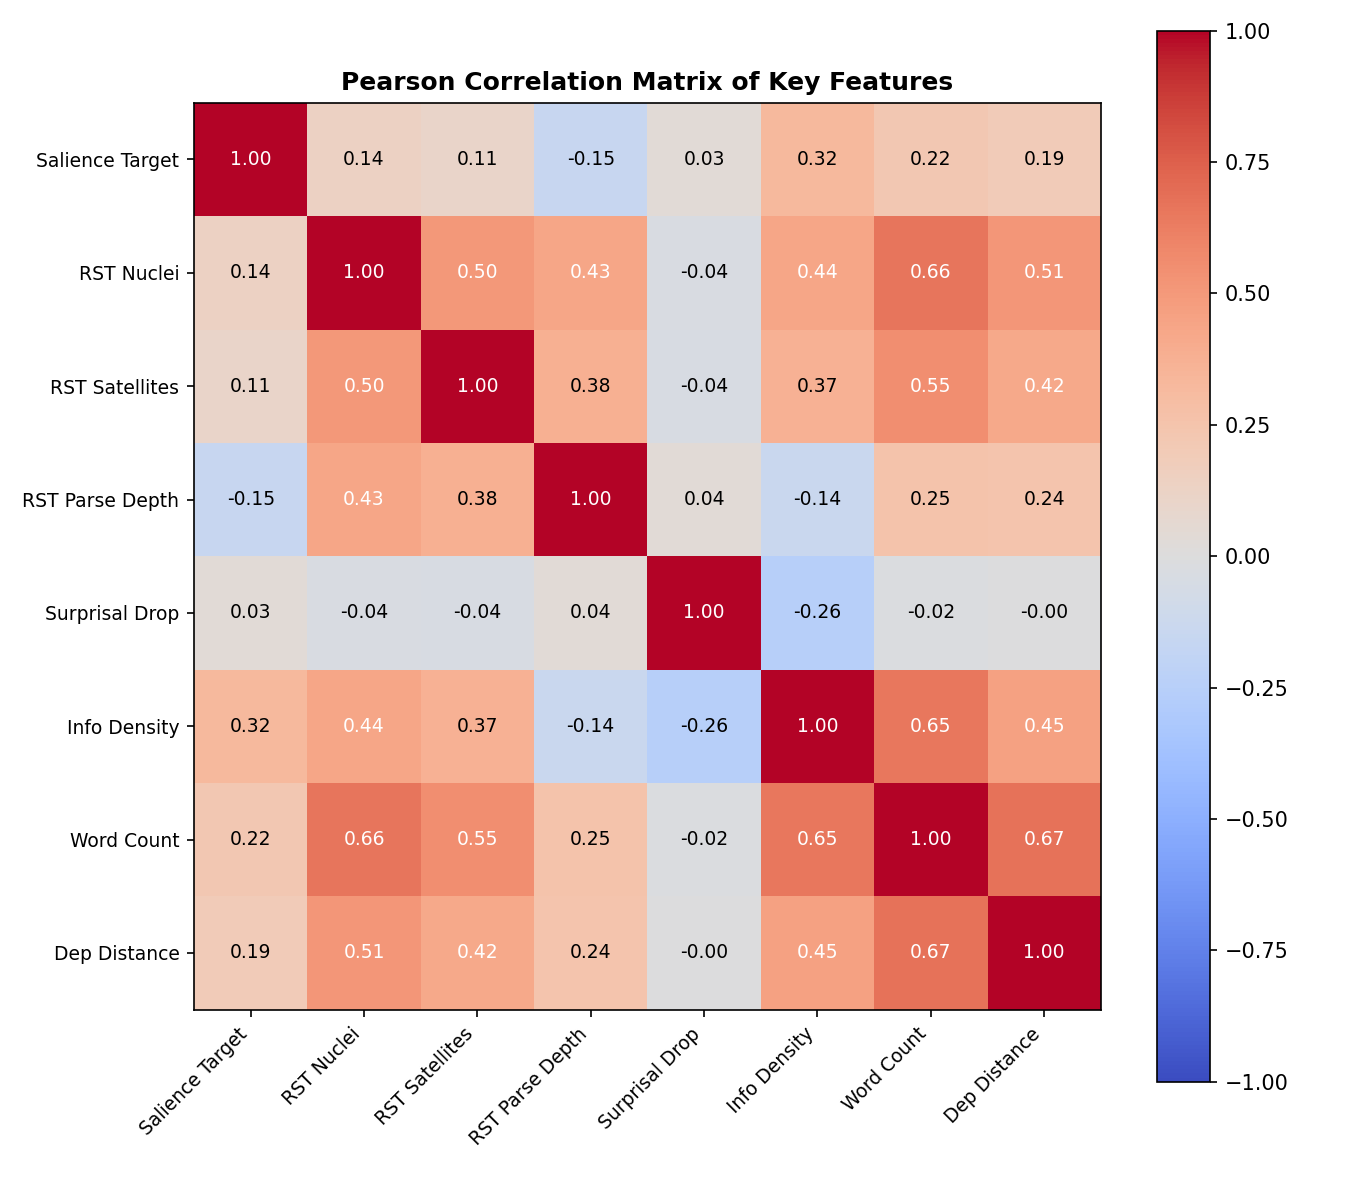
\includegraphics[width=\linewidth]{images/correlation_heatmap.png}
\caption{Feature correlation heatmap highlighting independence of RST and surprisal features.}
\label{fig:heatmap}
\end{figure}

\section{Conclusion}
We introduced DSNB neighborhood balancing and the LGSM convex-gated sequence transformer for sentence salience classification. Our empirical results prove that combining explicit RST discourse hierarchies with neural transformer embeddings effectively neutralizes positional shortcuts and outperforms zero-shot LLM judges.

\bibliographystyle{plain}
\begin{thebibliography}{99}
\bibitem{du2017learning} Xinya Du, Junru Shao, and Claire Cardie. 2017. Learning to Ask: Neural Question Generation for Reading Comprehension. In \textit{Proceedings of ACL}.
\bibitem{rajpurkar2016squad} Pranav Rajpurkar et al. 2016. SQuAD: 100,000+ Questions for Machine Comprehension of Text. In \textit{Proceedings of EMNLP}.
\bibitem{mann1988rhetorical} William C. Mann and Sandra A. Thompson. 1988. Rhetorical Structure Theory: Toward a functional theory of text organization. \textit{Text-Interdisciplinary Journal for the Study of Discourse}.
\bibitem{chistova2021isanlp} Elena Chistova et al. 2021. ISAnLP RST: Open-source neural parser for Rhetorical Structure Theory.
\bibitem{brysbaert2014concreteness} Marc Brysbaert, Amy Beth Warriner, and Victor Kuperman. 2014. Concreteness ratings for 40,000 generally known English word lemmas. \textit{Behavior Research Methods}.
\end{thebibliography}

\end{document}
